\documentclass[landscape,a0paper,fontscale=0.292]{baposter}

\usepackage[vlined]{algorithm2e}
\usepackage{times}
\usepackage{calc}
\usepackage{url}
\usepackage[pagebackref=true,breaklinks=true,letterpaper=true,colorlinks,bookmarks=false,urlcolor = blue,]{hyperref}
\usepackage{graphicx}
\usepackage{amsmath}
\usepackage{amssymb}
\usepackage{relsize}
\usepackage{multirow}
\usepackage{booktabs}

\usepackage{graphicx}
\usepackage{multicol}
\usepackage[T1]{fontenc}
\usepackage{ae}
\usepackage{enumitem}

\usepackage{colortbl}
\usepackage{xcolor}
\graphicspath{{images/}}

\setlist[itemize]{leftmargin=*,nosep}
 \setlength{\columnsep}{0.7em}
 \setlength{\columnseprule}{0mm}


% %%%%%%%%%%%%%%%%%%%%%%%%%%%%%%%%%%%%%%%%%%%%%%%%%%%%%%%%%%%%%%%%%%%%%%%%%%%%%%%%
% % Save space in lists. Use this after the opening of the list
% %%%%%%%%%%%%%%%%%%%%%%%%%%%%%%%%%%%%%%%%%%%%%%%%%%%%%%%%%%%%%%%%%%%%%%%%%%%%%%%%
 \newcommand{\compresslist}{%
 \setlength{\itemsep}{0pt}%
 \setlength{\parskip}{0pt}%
 \setlength{\parsep}{0pt}%
 }
\renewcommand{\rmdefault}{ptm} % Arial
\renewcommand{\sfdefault}{ptm} % Arial

\usepackage{bm} % for bold gamma

\DeclareMathOperator*{\argmin}{arg\,min}
\DeclareMathOperator*{\argmax}{arg\,max}
\def\support{\mbox{support}}
%% Italian Short Terms
\def\diag{\mbox{diag}}
\def\rank{\mbox{rank}}
\def\grad{\mbox{\text{grad}}}
\def\dist{\mbox{dist}}
\def\sgn{\mbox{sgn}}
\def\tr{\mbox{tr}}
\def\card{{\mbox{Card}}}

%%bold greek letters\bvarpi
\def\balpha{\mbox{{\boldmath $\alpha$}}}
\def\bbeta{\mbox{{\boldmath $\beta$}}}
\def\bzeta{\mbox{{\boldmath $\zeta$}}}
\def\bgamma{\mbox{{\boldmath $\gamma$}}}
\def\bdelta{\mbox{{\boldmath $\delta$}}}
\def\bmu{\mbox{{\boldmath $\mu$}}}
\def\bftau{\mbox{{\boldmath $\tau$}}}
\def\beps{\mbox{{\boldmath $\epsilon$}}}
\def\blambda{\mbox{{\boldmath $\lambda$}}}
\def\bLambda{\mbox{{\boldmath $\Lambda$}}}
\def\bnu{\mbox{{\boldmath $\nu$}}}
\def\bomega{\mbox{{\boldmath $\omega$}}}
\def\bfeta{\mbox{{\boldmath $\eta$}}}
\def\bsigma{\mbox{{\boldmath $\sigma$}}}
\def\bzeta{\mbox{{\boldmath $\zeta$}}}
\def\bphi{\mbox{{\boldmath $\phi$}}}
\def\bxi{\mbox{{\boldmath $\xi$}}}
\def\bvphi{\mbox{{\boldmath $\phi$}}}
\def\bdelta{\mbox{{\boldmath $\delta$}}}
\def\bvarpi{\mbox{{\boldmath $\varpi$}}}
\def\bvarsigma{\mbox{{\boldmath $\varsigma$}}}
\def\bXi{\mbox{{\boldmath $\Xi$}}}
\def\bmW{\mbox{{\boldmath $\mW$}}}
\def\bmY{\mbox{{\boldmath $\mY$}}}

\def\bPi{\mbox{{\boldmath $\Pi$}}}

\def\bOmega{\mbox{{\boldmath $\Omega$}}}
\def\bDelta{\mbox{{\boldmath $\Delta$}}}
\def\bPi{\mbox{{\boldmath $\Pi$}}}
% \def\bPsi{\mbox{{\boldmath $\Psi$}}}
\def\bSigma{\mbox{{\boldmath $\Sigma$}}}
\def\bUpsilon{\mbox{{\boldmath $\Upsilon$}}}

%%mathcal letters
\def\mA{{\mathcal A}}
\def\mB{{\mathcal B}}
\def\mC{{\mathcal C}}
\def\mD{{\mathcal D}}
\def\mE{{\mathcal E}}
\def\mF{{\mathcal F}}
\def\mG{{\mathcal G}}
\def\mH{{\mathcal H}}
\def\mI{{\mathcal I}}
\def\mJ{{\mathcal J}}
\def\mK{{\mathcal K}}
\def\mL{{\mathcal L}}
\def\mM{{\mathcal M}}
\def\mN{{\mathcal N}}
\def\mO{{\mathcal O}}
\def\mP{{\mathcal P}}
\def\mQ{{\mathcal Q}}
\def\mR{{\mathcal R}}
\def\mS{{\mathcal S}}
\def\mT{{\mathcal T}}
\def\mU{{\mathcal U}}
\def\mV{{\mathcal V}}
\def\mW{{\mathcal W}}
\def\mX{{\mathcal X}}
\def\mY{{\mathcal Y}}
\def\mZ{{\mathcal{Z}}}



%%bold mathcal letters
\DeclareMathAlphabet\mathbfcal{OMS}{cmsy}{b}{n}
%bold mathcal letters
\def\bmA{{\mathbfcal A}}
\def\bmB{{\mathbfcal B}}
\def\bmC{{\mathbfcal C}}
\def\bmD{{\mathbfcal D}}
\def\bmE{{\mathbfcal E}}
\def\bmF{{\mathbfcal F}}
\def\bmG{{\mathbfcal G}}
\def\bmH{{\mathbfcal H}}
\def\bmI{{\mathbfcal I}}
\def\bmJ{{\mathbfcal J}}
\def\bmK{{\mathbfcal K}}
\def\bmL{{\mathbfcal L}}
\def\bmM{{\mathbfcal M}}
\def\bmN{{\mathbfcal N}}
\def\bmO{{\mathbfcal O}}
\def\bmP{{\mathbfcal P}}
\def\bmQ{{\mathbfcal Q}}
\def\bmR{{\mathbfcal R}}
\def\bmS{{\mathbfcal S}}
\def\bmT{{\mathbfcal T}}
\def\bmU{{\mathbfcal U}}
\def\bmV{{\mathbfcal V}}
\def\bmW{{\mathbfcal W}}
\def\bmX{{\mathbfcal X}}
\def\bmY{{\mathbfcal Y}}
\def\bmZ{{\mathbfcal Z}}



%%bold letters
\def\0{{\bf 0}}
\def\1{{\bf 1}}

%%bold capital Cases
\def\bA{{\bf A}}
\def\bB{{\bf B}}
\def\bC{{\bf C}}
\def\bD{{\bf D}}
\def\bE{{\bf E}}
\def\bF{{\bf F}}
\def\bG{{\bf G}}
\def\bH{{\bf H}}
\def\bI{{\bf I}}
\def\bJ{{\bf J}}
\def\bK{{\bf K}}
\def\bL{{\bf L}}
\def\bM{{\bf M}}
\def\bN{{\bf N}}
\def\bO{{\bf O}}
\def\bP{{\bf P}}
\def\bQ{{\bf Q}}
\def\bR{{\bf R}}
\def\bS{{\bf S}}
\def\bT{{\bf T}}
\def\bU{{\bf U}}
\def\bV{{\bf V}}
\def\bW{{\bf W}}
\def\bX{{\bf X}}
\def\bY{{\bf Y}}
\def\bZ{{\bf{Z}}}


%%bold small cases
\def\ba{{\bf a}}
\def\bb{{\bf b}}
\def\bc{{\bf c}}
\def\bd{{\bf d}}
\def\be{{\bf e}}
\def\bff{{\bf f}}
\def\bg{{\bf g}}
\def\bh{{\bf h}}
\def\bi{{\bf i}}
\def\bj{{\bf j}}
\def\bk{{\bf k}}
\def\bl{{\bf l}}
%\def\bm{{\bf m}}
\def\bn{{\bf n}}
\def\bo{{\bf o}}
\def\bp{{\bf p}}
\def\bq{{\bf q}}
\def\br{{\bf r}}
\def\bs{{\bf s}}
\def\bt{{\bf t}}
\def\bu{{\bf u}}
\def\bv{{\bf v}}
\def\bw{{\bf w}}
\def\bx{{\bf x}}
\def\by{{\bf y}}
\def\bz{{\bf z}}

%%hat letters
\def\hy{\hat{y}}
\def\hby{\hat{{\bf y}}}


%%mathrm letters
\def\mmE{{\mathbb E}}
\def\mmP{{\mathrm P}}
\def\mmB{{\mathrm B}}
\def\mmR{{\mathbb R}}
\def\mmV{{\mathbb V}}
\def\mmN{{\mathbb N}}
\def\mmZ{{\mathbb Z}}
\def\mMLr{{\mM_{\leq k}}}
\def\mmI{{\mathbb I}}
\def\mmS{{\mathbb S}}
\def\mmL{{\mathbb L}}

%%tidle cases
\def\tC{\tilde{C}}
\def\tk{\tilde{r}}
\def\tJ{\tilde{J}}
\def\tbx{\tilde{\bx}}
\def\tbK{\tilde{\bK}}
\def\tL{\tilde{L}}
\def\tbPi{\mbox{{\boldmath $\tilde{\Pi}$}}}
\def\tw{{\bf \tilde{w}}}



%%bar cases
\def\barx{\bar{\bx}}

%%terms for short
\def\pd{{\succ\0}}
\def\psd{{\succeq\0}}
\def\vphi{\varphi}
\def\trsp{{\sf T}}

%short phrase
\def\mRMD{{\mathrm{D}}}
\def \DKL{{D_{KL}}}
\def\st{{\mathrm{s.t.}}}
\def\nth{{\mathrm{th}}}


\def\bx{{\bf x}}
\def\bX{{\bf X}}
\def\by{{\bf y}}
\def\bY{{\bf Y}}
\def\bw{{\bf w}}
\def\bW{{\bf W}}
\def\balpha{{\bm \alpha}}
\def\bbeta{{\bm \beta}}
\def\boldeta{{\bm \eta}}
\def\boldEta{{\bm \Eta}}
\def\bgamma{{\bm \gamma}}
\def\bGamma{{\bm \Gamma}}
\def\bmu{{\bm \mu}}
\def\bbeta{{\bm \beta}}

\def\bK{{\bf K}}
\def\bb{{\bf b}}
\def\bg{{\bf g}}
\def\bp{{\bf p}}
\def\bP{{\bf P}}
\def\bh{{\bf h}}
\def\bc{{\bf c}}
\def\bz{{\bf z}}
% \def\bm{{\bf m}}

\def\st{{\mathrm{s.t.}}}
\def\tr{\mathrm{tr}}
\def\grad{{\mathrm{grad}}}

\newtheorem{coll}{Corollary}
\newtheorem{deftn}{Definition}
\newtheorem{thm}{Theorem}
\newtheorem{prop}{Proposition}
% \newtheorem{lemma}{Lemma}
% \newtheorem{remark}{Remark}
% \newtheorem{ass}{Assumption}
% \newtheorem{proof}{Proof}

\newcommand{\tabincell}[2]{\begin{tabular}{@{}#1@{}}#2\end{tabular}}

\def\eg{\emph{e.g.,}} \def\Eg{\emph{E.g.}}
\def\ie{\emph{i.e.,}} \def\Ie{\emph{I.e.}}
\def\cf{\emph{c.f.}} \def\Cf{\emph{C.f.}}
\def\etc{\emph{etc.}} \def\vs{\emph{vs.}}
\def\wrt{{w.r.t.}} \def\dof{d.o.f}
\def\etal{{\em et al.\/}\,}

\newcommand{\name}{Densely-Anchored Sampling\xspace}
\newcommand{\shortname}{DAS\xspace}
\newcommand{\lowername}{densely-anchored sampling\xspace}

\newcommand{\bfs}{Discriminative Feature Scaling\xspace}
\newcommand{\shortbfs}{DFS\xspace}

\newcommand{\tmb}{Memorized Transformation Shifting\xspace}
\newcommand{\shorttmb}{MTS\xspace}

%%%%%%%%%%%%%%%%%%%%%%%%%%%%%%%%%%%%%%%%%%%%%%%%%%%%%%%%%%%%%%%%%%%%%%%%%%%%%
%% Begin of Document
%%%%%%%%%%%%%%%%%%%%%%%%%%%%%%%%%%%%%%%%%%%%%%%%%%%%%%%%%%%%%%%%%%%%%%%%%%%%%
\begin{document}
%%%%%%%%%%%%%%%%%%%%%%%%%%%%%%%%%%%%%%%%%%%%%%%%%%%%%%%%%%%%%%%%%%%%%%%%%%%%%
%% Here starts the poster
%%---------------------------------------------------------------------------
%% Format it to your taste with the options
%%%%%%%%%%%%%%%%%%%%%%%%%%%%%%%%%%%%%%%%%%%%%%%%%%%%%%%%%%%%%%%%%%%%%%%%%%%%%
\begin{poster}{
 % Show grid to help with alignment
 grid=false,
 columns=5,
 % Column spacing
 colspacing=0.7em,
 % Color style
 headerColorOne=cyan!20!white!90!black,
 borderColor=cyan!30!white!90!black,
 % Format of textbox
 textborder=faded,
 % Format of text header
 headerborder=open,
 headershape=roundedright,
 headershade=plain,
 background=none,
 bgColorOne=cyan!10!white,
 headerheight=0.12\textheight}
 % Eye Catcher
 {
      
\includegraphics[width=0.08\linewidth]{images/SCUT_logo.jpg}
      \makebox[0.01\textwidth]{}
      % \raisebox{0.08\height}
      {
\includegraphics[width=0.08\linewidth]{images/PCL_logo.jpg}}
      \makebox[0.04\textwidth]{} 
 }
 % Title
 {\sc\huge\bf \name for Deep Metric Learning}
 % Authors
 % {\vspace{0.3em} Lizhao Liu$^{1,2}$, Shangxin Huang$^1$, Zhuangwei Zhuang$^1$, Ran Yang$^1$, Mingkui Tan$^{1,3\dag}$, and Yaowei Wang$^{2\dag}$ \\[0.2em]
 % {$^1$South China University of Technology $^2$PengCheng Laboratory \\ $^3$Key Laboratory of Big Data and Intelligent Robot, Ministry of Education \\[0.2em] ($\dag$ indicates the corresponding author)}}
  {\vspace{0.3em} Lizhao Liu$^{1,2}$, Shangxin Huang$^1$, Zhuangwei Zhuang$^1$, Ran Yang$^1$, Mingkui Tan$^{1,3}$, and Yaowei Wang$^{2}$ \\[0.2em]
 {$^1$South China University of Technology $^2$PengCheng Laboratory \\ $^3$Key Laboratory of Big Data and Intelligent Robot, Ministry of Education \\[0.2em]}}
 %{\texttt{\{gychen, khan, kykwong\}@cs.hku.hk}}}
 % University logo
 {
  \begin{tabular}{r}
    \makebox[0.01\textwidth]{}
    % 
\includegraphics[width=0.12\linewidth]{images/ECCV_logo.png}
    % 
\includegraphics[width=0.12\linewidth]{images/eccv-logo-big-black.png}
    
\includegraphics[width=0.12\linewidth]{images/ECCV-logo3.png}
  \end{tabular}
 }

%%%%%%%%%%%%%%%%%%%%%%%%%%%%%%%%%%%%%%%%%%%%%%%%%%%%%%%%%%%%%%%%%%%%%%%%%%%%%%
%%% Now define the boxes that make up the poster
%%%---------------------------------------------------------------------------
%%% Each box has a name and can be placed absolutely or relatively.
%%% The only inconvenience is that you can only specify a relative position 
%%% towards an already declared box. So if you have a box attached to the 
%%% bottom, one to the top and a third one which should be inbetween, you 
%%% have to specify the top and bottom boxes before you specify the middle 
%%% box.
%%%%%%%%%%%%%%%%%%%%%%%%%%%%%%%%%%%%%%%%%%%%%%%%%%%%%%%%%%%%%%%%%%%%%%%%%%%%%%

%%%%%%%%%%%%%%%%%%%%%%%%%%%%%%%%%%%%%%%%%%%%%%%%%%%%%%%%%%%%%%%%%%%%%%%%%%%%%%
\headerbox{\bf\color{blue} Problem Definition and Contribution}{name=contribution,column=0,row=0,span=2}{
   \textbf{\color{blue}Goal:} To train a deep model that projects semantically similar data into nearby embedding space, Deep Metric Learning (DML) methods often highly depends on sampling effective data from the embedding space.
    
    \vspace{0.2em}
    \textbf{\color{blue}Key Contributions:} A PnP \name (\shortname) scheme for DML that
    \begin{itemize}
      \item exploits embeddings’ nearby embedding space and densely produces embeddings.
      \item includes two models, namely \bfs (\shortbfs) and \tmb (\shorttmb). 
      \item consistently improves existing DML baselines without bells and whistles.
    \end{itemize}  
}


%%%%%%%%%%%%%%%%%%%%%%%%%%%%%%%%%%%%%%%%%%%%%%%%%%%%%%%%%%%%%%%%%%%%%%%%%%%%%
\headerbox{\bf\color{blue} Experiments \& Results}{name=results,column=2,row=0,span=3}{
    \textbf{\color{blue}Dataset:}

    \vspace{0.5em}
    \begin{minipage}{\linewidth}
        We use three popular benchmarks:
        \begin{itemize}
            \item CUB2011-200 (CUB), a fine-grained bird dataset, \#Train~/~\#Test classes: 100~/~100.
            \item CARS196 (CARS), a fine-grained vehicle dataset, \#Train~/~\#Test classes: 98~/~98.
            \item Stanford Online Products (SOP), a large-scale online products dataset, \#Train~/~\#Test classes: 11,318~/~11,316.
        \end{itemize}
    \end{minipage}

   \vspace{1.0em}
    \begin{minipage}{0.44\linewidth}
        \centering
        \textbf{\color{blue}Improvements over Pair-based Methods:}

        \vspace{0.2em}
        \resizebox{\textwidth}{!}{
\Huge
\begin{tabular}{l|ccc|ccc|ccc}
% 		\topline
    \toprule
    \multirow{2}[0]{*}{Method} & \multicolumn{3}{c|}{CUB} & \multicolumn{3}{c|}{CARS} & \multicolumn{3}{c}{SOP} \\ \cline{2-10} % \cmidrule(r){3-11}
    & R@1 & F1 & NMI & R@1 & F1 & NMI & R@1 & F1 & NMI \\
    \midrule
    Triplet [S] & 60.25 & 32.82 & 64.64 & 74.64 & 31.98 & 63.22 & 73.51 & 33.47 & 89.33 \\
    Triplet [S] {+ \shortname} & \textbf{60.82} & \textbf{33.86} & \textbf{65.67} & \textbf{77.21} & \textbf{33.88} & \textbf{64.84} & \textbf{73.99} & \textbf{33.91} & \textbf{89.42}  \\
    \midrule
    Triplet [D] & 62.68 & 36.39 & 67.03 & 78.86 & 35.80 & 65.85 & 77.54 & 37.10 & 90.05 \\
    Triplet [D] {+ \shortname} & \textbf{64.28} & \textbf{38.16} & \textbf{68.06} & \textbf{82.63} & \textbf{39.14} & \textbf{68.12} & \textbf{77.95} & \textbf{37.64} & \textbf{90.18} \\
    \midrule
    Contrastive [D] & 61.65 & 35.23 & 66.58 & 76.03 & 32.77 & 64.09 & 73.13 & 35.60 & 89.78 \\
    Contrastive [D] {+ \shortname} & \textbf{63.67} & \textbf{36.25} & \textbf{67.15} &
    \textbf{80.74} & \textbf{36.07} & \textbf{65.93} & \textbf{74.80} & \textbf{36.21} & \textbf{89.89} \\
    \midrule
    Margin & 62.61 & 37.33 & 67.58 &
    80.10 & 37.85 & 67.15 & 78.69 & 39.20 & 90.50 \\
    Margin {+ \shortname} & \textbf{64.50} & \textbf{37.86} & \textbf{68.04} &
    \textbf{82.29} & \textbf{38.22} & \textbf{67.94} & \textbf{79.14} & \textbf{39.52} & \textbf{90.56} \\ %TODO 
    \midrule
    GenLifted & 58.81 & 34.64 & 65.50 & 72.45 & 32.43 & 64.00 & 76.18 & 37.26 & 90.13 \\
    GenLifted {+ \shortname} & \textbf{59.94} & \textbf{35.09} & \textbf{66.07} &
    \textbf{73.55} & \textbf{32.85} & \textbf{64.11} & \textbf{76.92} & \textbf{37.64} & \textbf{90.21} \\
    \midrule
    N-Pair & 60.55 & 36.94 & 67.19 & 77.35 & 36.26 & 66.74 & 77.71 & 37.13 & 90.15 \\
    N-Pair {+ \shortname} & \textbf{62.81} & \textbf{38.37} & \textbf{68.43} & \textbf{79.93} & \textbf{38.06} & \textbf{68.20} & \textbf{77.98} & \textbf{37.82} & \textbf{90.28} \\
    \midrule
    MS & 62.63 & 38.88 & 68.19 & 82.04 & 40.85 & 69.45 & 78.89 & 37.53 & 90.12 \\
    MS {+ \shortname} & \textbf{64.13} & \textbf{39.18} & \textbf{69.08} &
    \textbf{83.31} & \textbf{42.78} & \textbf{70.77} & \textbf{79.44} & \textbf{38.77} & \textbf{90.40} \\
\bottomrule
\end{tabular}
}
    \end{minipage}
    % \hdashline
    \begin{minipage}{0.52\linewidth}
        \centering
        \textbf{\color{blue}Comparison with State-of-The-Arts:}

        \vspace{0.2em}
        \newcommand{\na}{\text{N/A}}

\resizebox{\linewidth}{!}{
\Huge{
	\begin{tabular}{lc|cccc|cccc|cccc}
% 		\topline
		\toprule
		\multirow{2}{*}{Method} & \multirow{2}{*}{Backbone} & \multicolumn{4}{c|}{CUB} & \multicolumn{4}{c|}{CARS} & \multicolumn{4}{c}{SOP} \\ 
        \cline{3-14} & & R@1 & R@2 & R@4 & R@8 & R@1 & R@2 & R@4 & R@8 & R@1 & R@10 & R@100 & R@1000  \\
        \midrule
		Margin & $\operatorname{R}^{128}$ & 63.60 & 74.40 & 83.10 & 90.00 & 79.60 & 86.50 & 91.90 & 95.10 & 72.70 & 86.20 & 93.80 & 98.00 \\
        HDC & $\operatorname{G}^{384}$ & 53.60 & 65.70 & 77.00 & 85.60 & 73.70 & 83.20 & 89.50 & 93.80 & 69.50 & 84.40 & 92.80 & 97.70 \\
        A-BIER & $\operatorname{G}^{384}$ & 57.50 & 68.70 & 78.30 & 86.20 & 82.00 & 89.00 & 93.20 & 96.10 & 74.20 & 86.90 & 94.00 & 97.80 \\
        ABE & $\operatorname{G}^{512}$ & 60.60 & 71.50 & 79.80 & 87.40 & 85.20 & 90.50 & 94.00 & 96.10 & 76.30 & 88.40 & 94.80 & 98.20 \\
        HTL & $\operatorname{IBN}^{512}$ & 57.10 & 68.80 & 78.70 & 86.50 & 81.40 & 88.00 & 92.70 & 95.70 & 74.80 & 88.30 & 94.80 & 98.40 \\
        RLL-H & $\operatorname{IBN}^{512}$ & 57.40 & 69.70 & 79.20 & 86.90 & 74.00 & 83.60 & 90.10 & 94.10 & 76.10 & 89.10 & 95.40 & \na \\
        SoftTriple & $\operatorname{IBN}^{512}$ & 65.40 & 76.40 & 84.50 & 90.40 & 84.50 & 90.70 & 94.50 & 96.90 & 78.30 & 90.30 & 95.90 & \na \\
        MS & $\operatorname{IBN}^{512}$ & 65.70 & 77.00 & 86.30 & 91.20 & 84.10 & 90.40 & 94.00 & 96.50 & 78.20 & 90.50 & 96.00 & 98.70 \\
        ProxyGML & $\operatorname{IBN}^{512}$ & 66.60 & 77.60 & 86.40 & \na & 85.50 & 91.80 & 95.30 & \na & 78.00 & 90.60 & 96.20 & \na \\
        ProxyAnchor & $\operatorname{IBN}^{512}$ & 68.40 & 79.20 & 86.80 & 91.60 & 86.10 & 91.70 & 95.00 & 97.30 & 79.10 & 90.80 & 96.20 & 98.70 \\
        \midrule
        Contrastive + XBM & $\operatorname{IBN}^{512}$ & 65.80 & 75.90 & 84.00 & 89.90 & 82.00 & 88.70 & 93.10 & 96.10 & 79.50 & 90.80 & 96.10 & 98.70 \\
        MS$^*$ & $\operatorname{IBN}^{512}$ & 64.50 & 76.20 & 84.60 & 90.50 & 82.10 & 88.80 & 93.20 & 96.10 & 76.30 & 89.70 & 96.00 & 98.80 \\
        MS + EE$^*$ & $\operatorname{IBN}^{512}$ & 65.10 & 76.80 & 86.10 & 91.00 & 82.70 & 89.20 & 93.80 & 96.40 & 77.00 & 89.50 & 96.00 & 98.80 \\
        ProxyAnchor + MemVir & $\operatorname{IBN}^{512}$ & 69.00 & 79.20 & 86.80 & 91.60 & 86.70 & 92.00 & 95.20 & 97.40 & 79.70 & 91.00 & 96.30 & 98.60 \\
        % \midline
        \midrule
        MS$^\dag$ & $\operatorname{IBN}^{512}$ & 65.72 & 77.19 & 85.74 & 91.56 & 83.86 & 90.41 & 94.64 & 96.99 & 76.89 & 89.58 & 95.59 & 98.60 \\
        MS + \shortname (Ours) & $\operatorname{IBN}^{512}$ & 67.07 & 78.11 & 86.43 & 91.88 & 85.66 & 91.60 & 95.27 & 97.37 & 78.16 & 90.26 & 95.99 & 98.76 \\
        MS$^\dag$ & $\operatorname{R}^{512}$ & 66.46 & 77.28 & 85.85 & 91.69 & 83.99 & 90.39 & 94.51 & 96.80 & 79.53 & 91.06 & 96.30 & 98.83 \\
        MS + \shortname (Ours) & $\operatorname{R}^{512}$ & \textbf{69.19} & \textbf{79.25} & \textbf{87.09} & \textbf{92.62} & \textbf{87.84} & \textbf{93.15} & \textbf{95.99} & \textbf{97.85} & \textbf{80.59} & \textbf{91.80} & \textbf{96.68} & \textbf{98.95} \\
        \bottomrule
	\end{tabular}
 }
}
    \end{minipage}

    \vspace{1.0em}
    \begin{minipage}{.66\linewidth}
        \centering
        \textbf{\color{blue}Experiments on Different Batch Size:}

        \vspace{0.2em}
        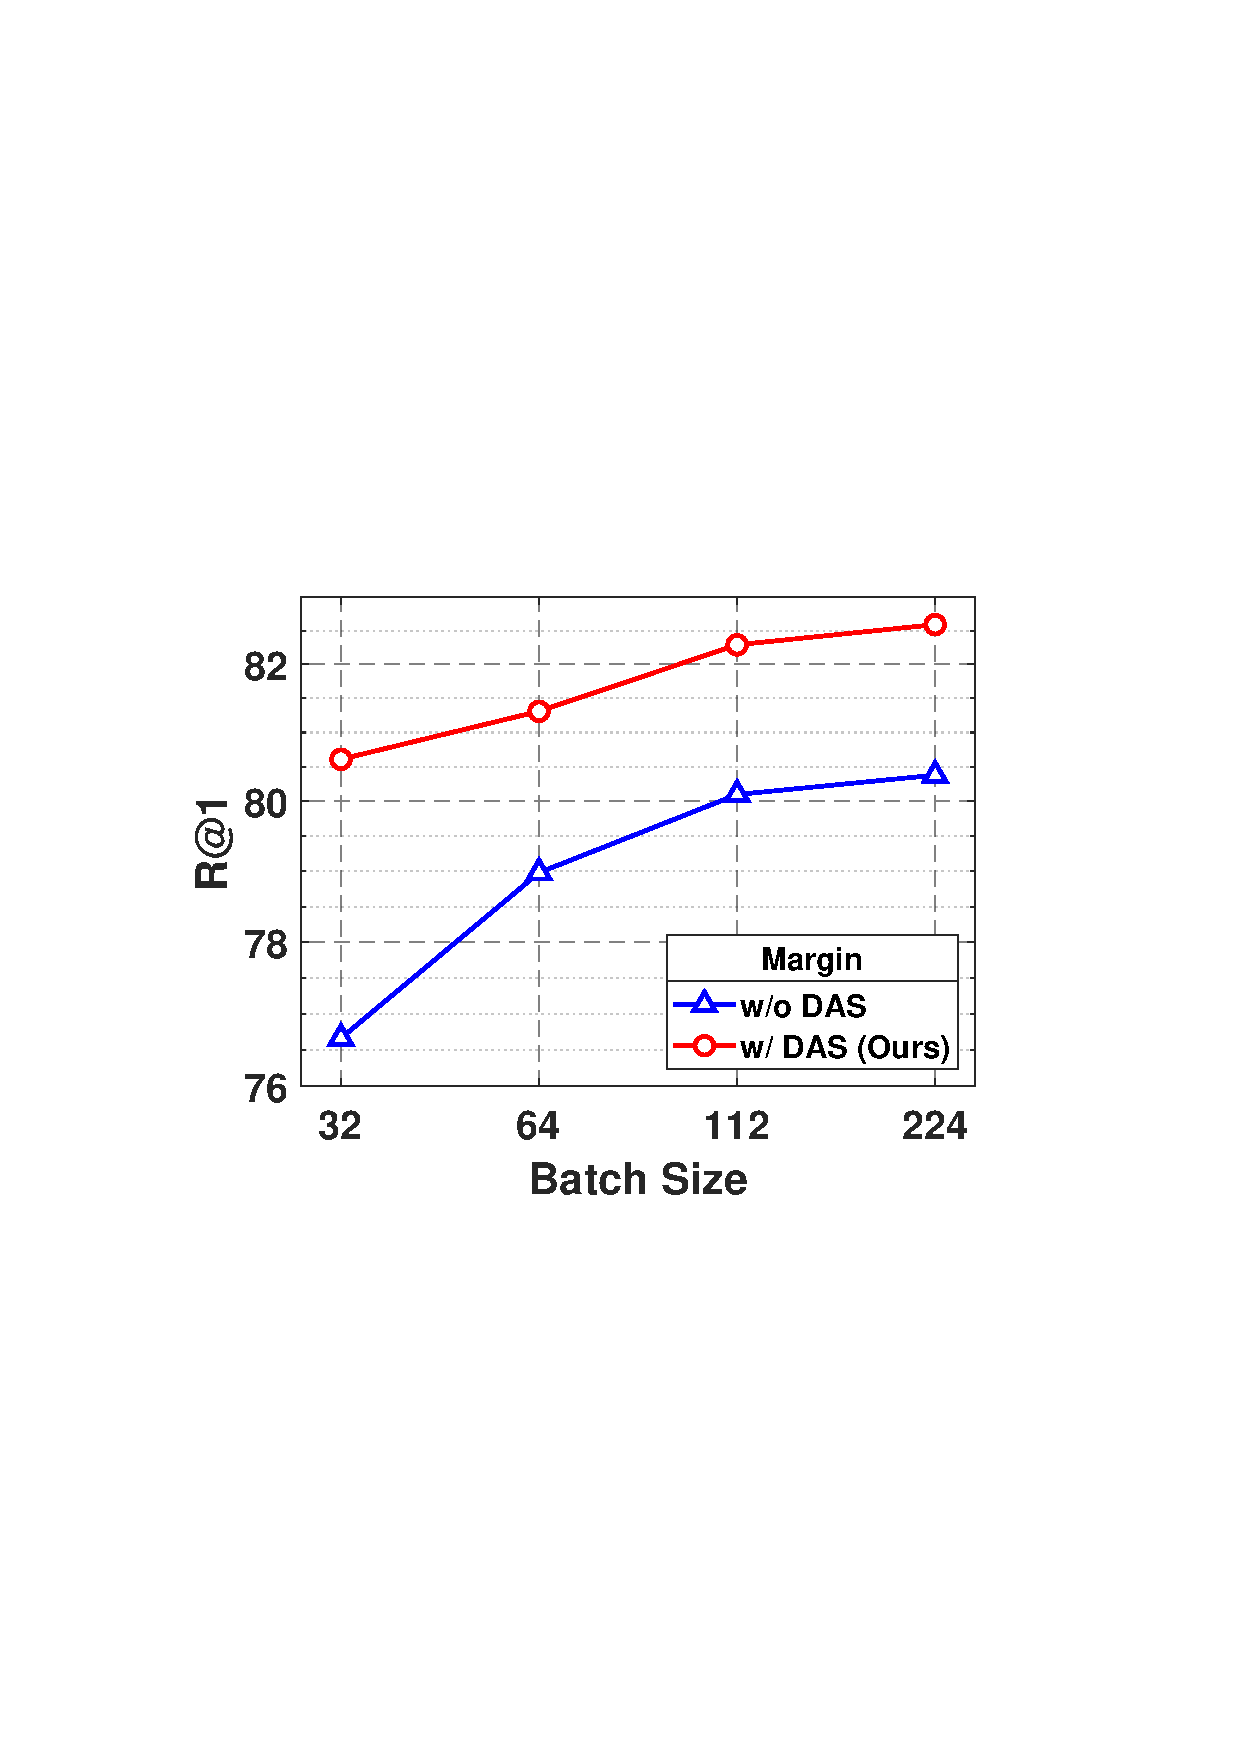
\includegraphics[width=.24\textwidth]{images/BS_R1.pdf}
        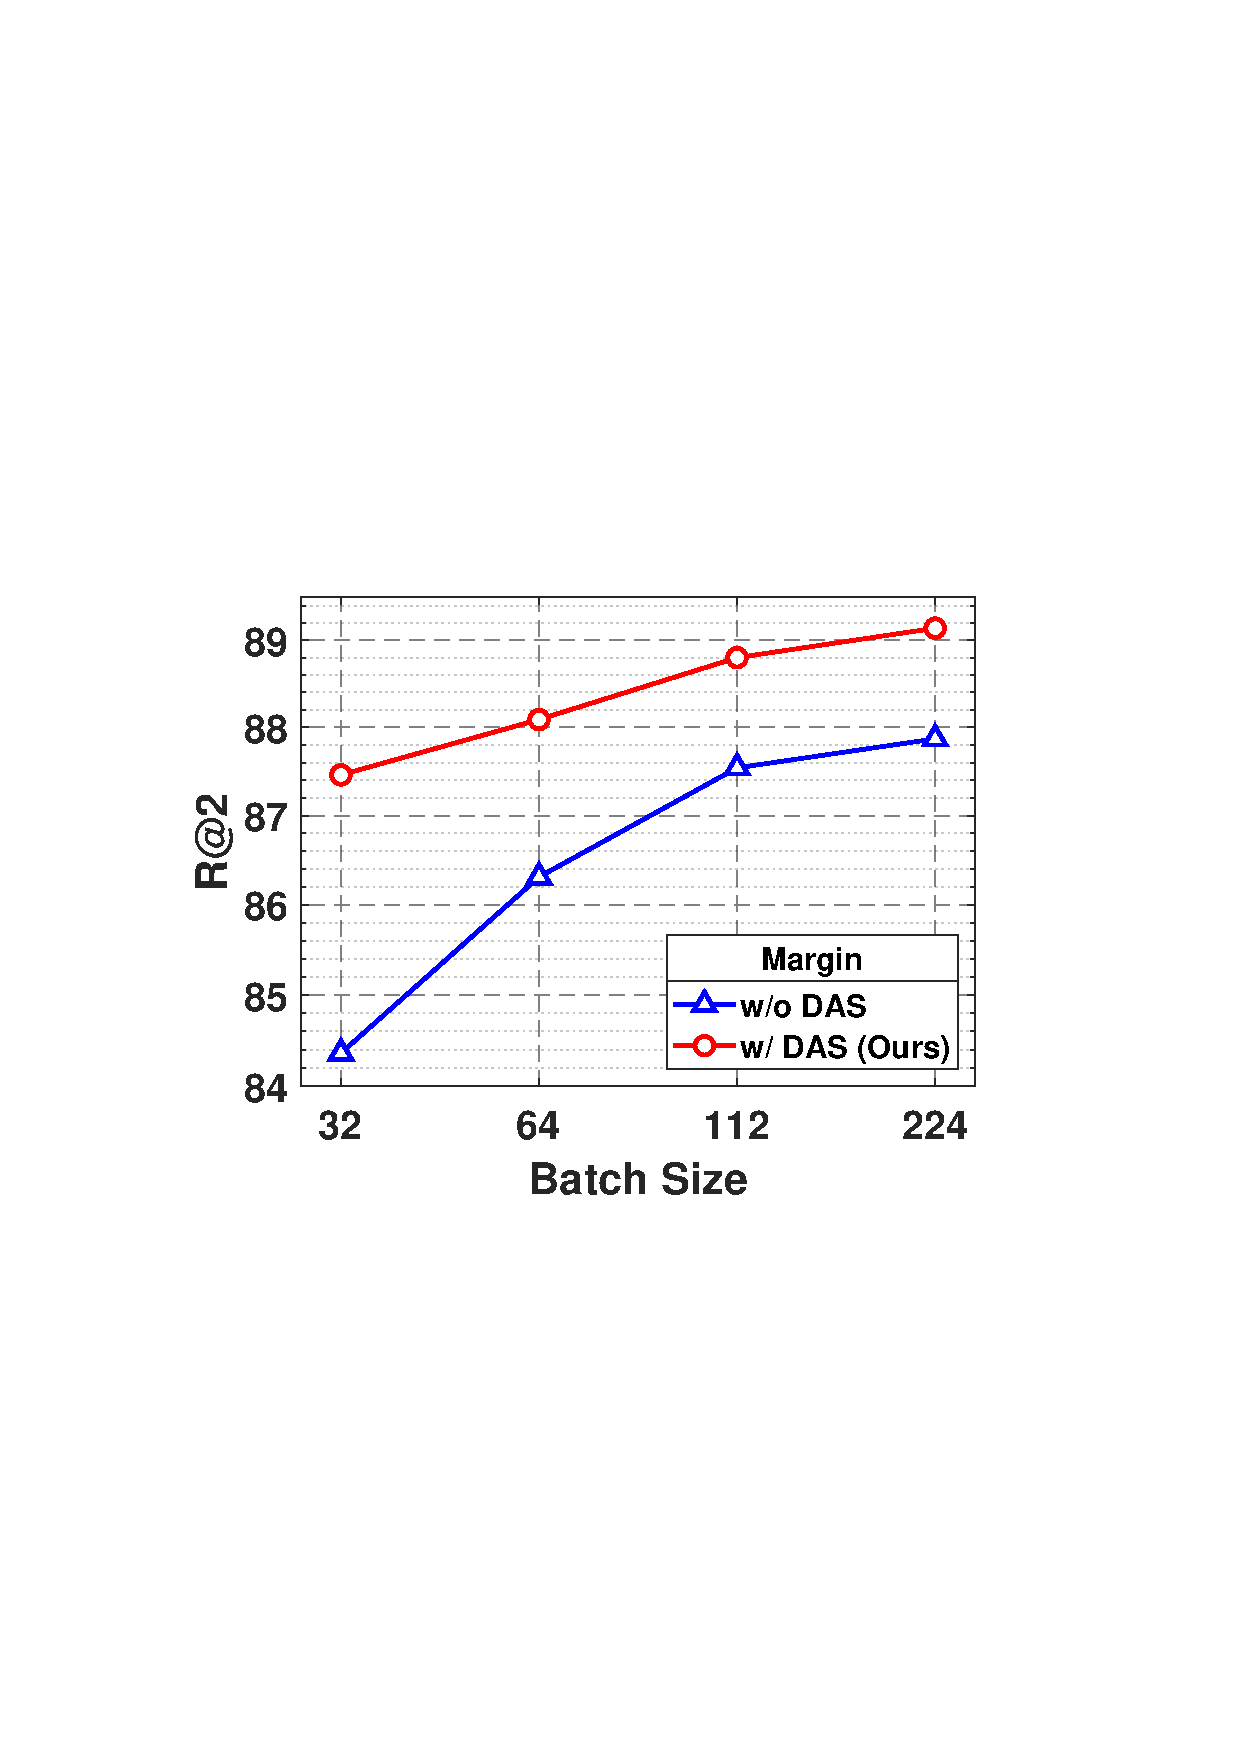
\includegraphics[width=.24\textwidth]{images/BS_R2.pdf}
        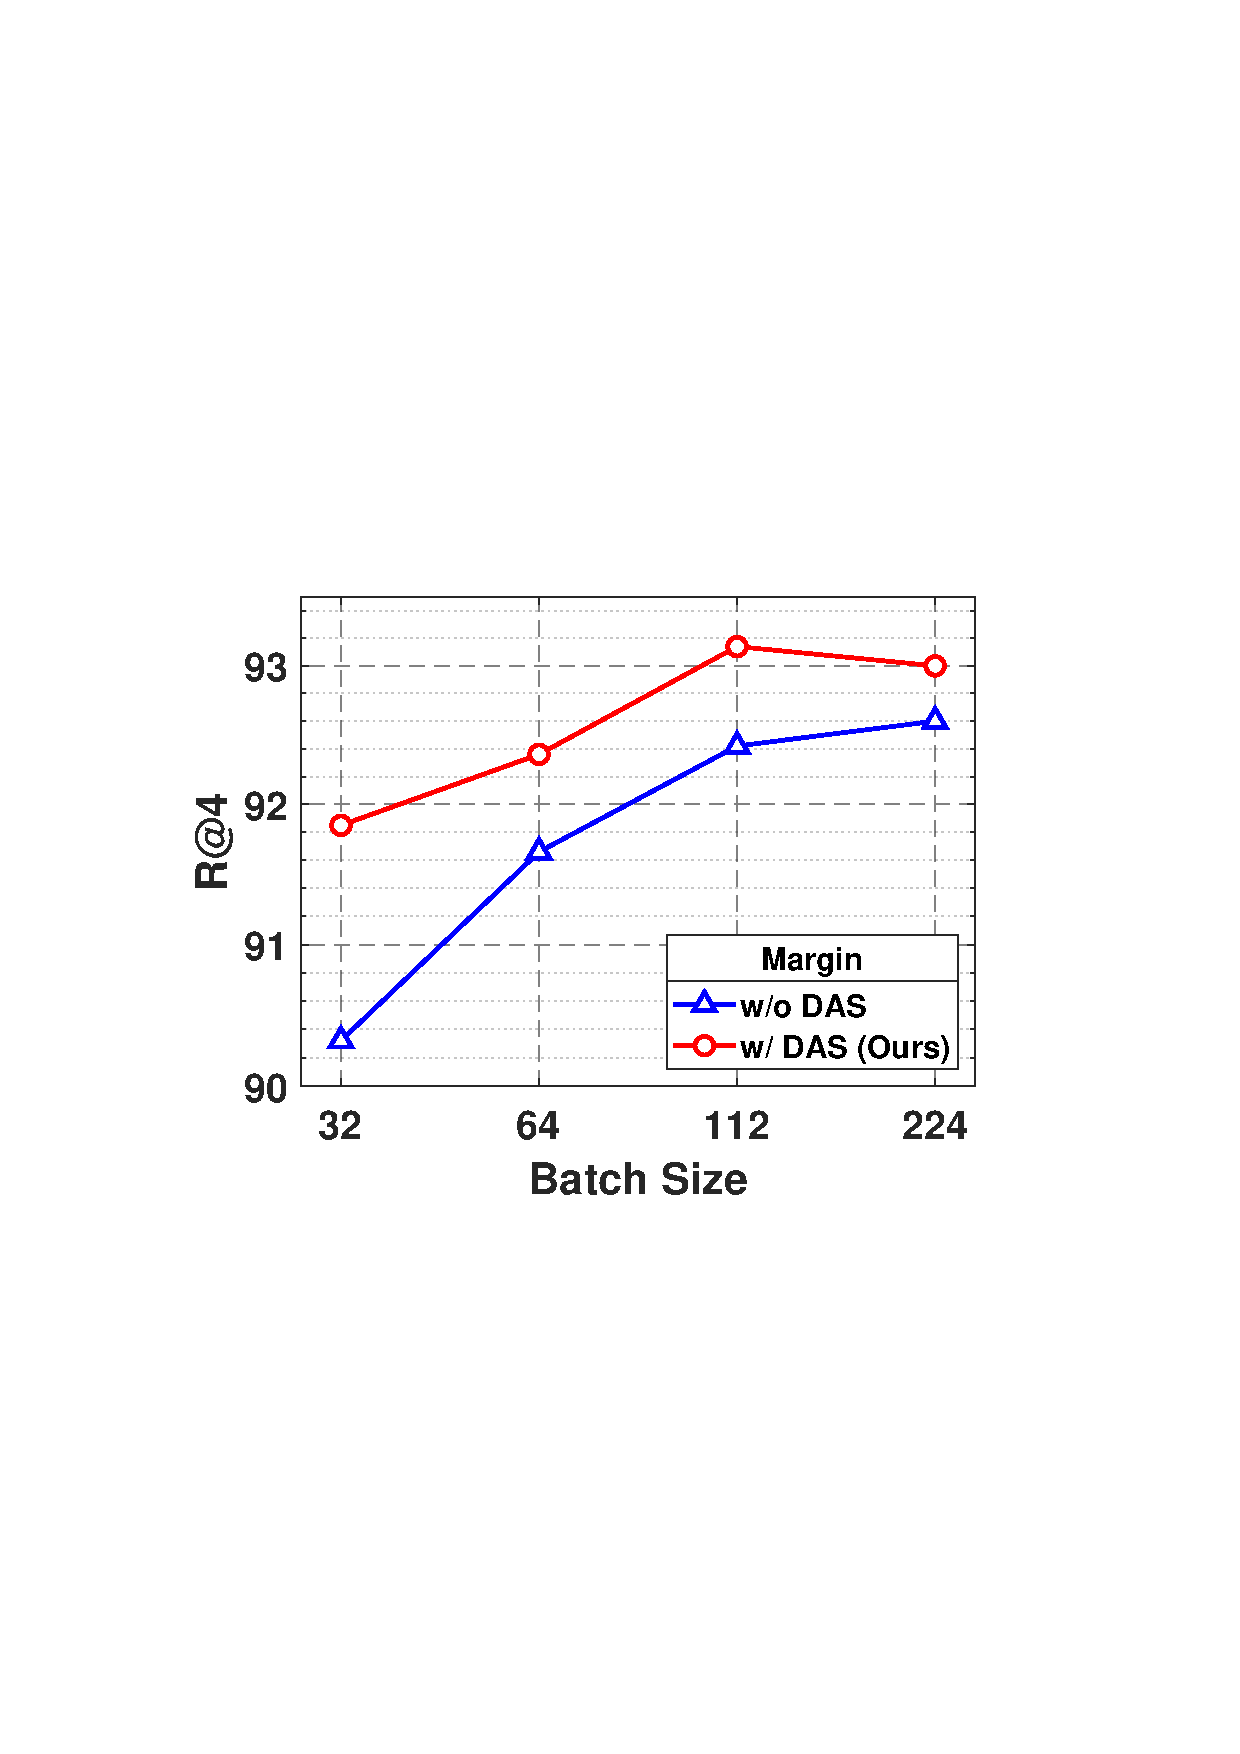
\includegraphics[width=.24\textwidth]{images/BS_R4.pdf}
        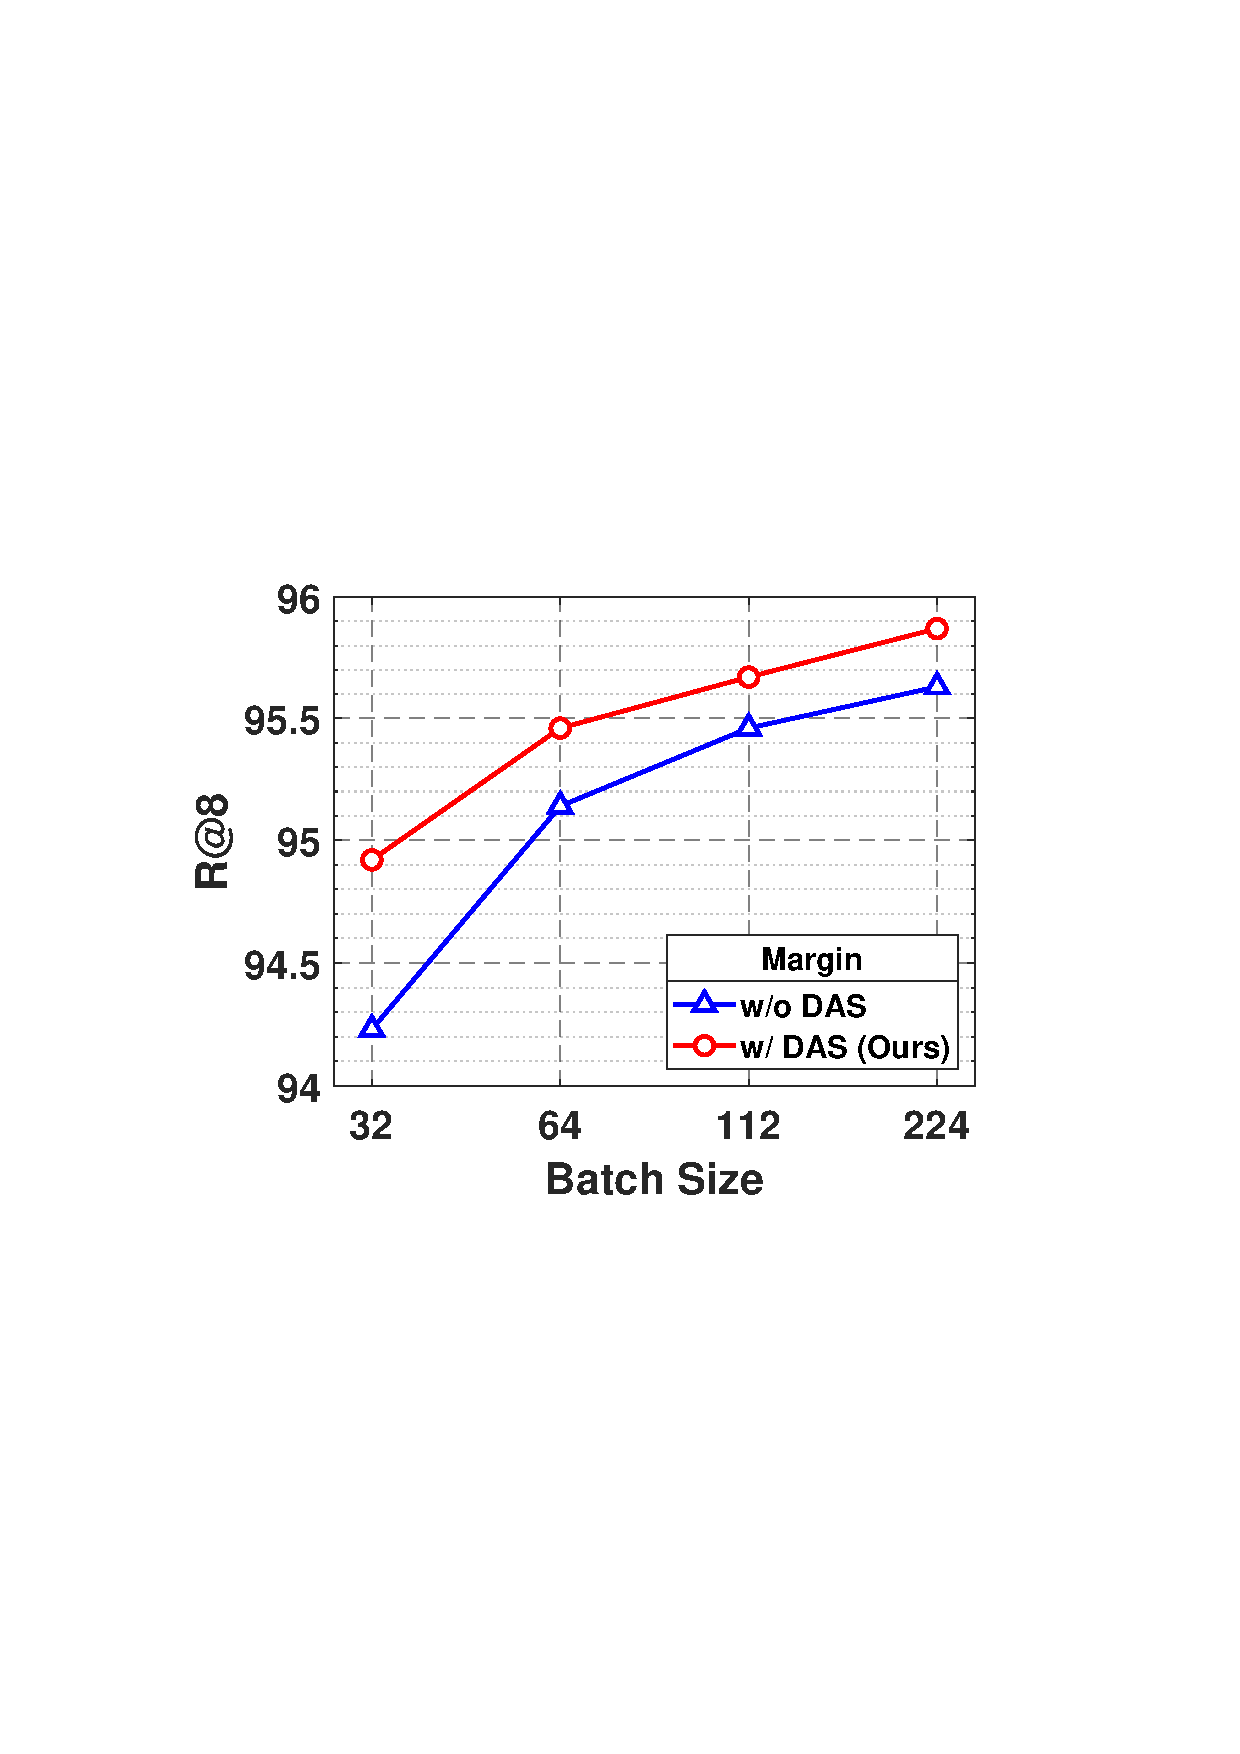
\includegraphics[width=.24\textwidth]{images/BS_R8.pdf}
        % \subcaption{Experiments using different batch size.}
    \end{minipage}
    \begin{minipage}[t]{0.33\linewidth}
        \vspace{-4.3em}
        \centering
        \textbf{\color{blue}Evolution of Training Process:}

        \vspace{0.2em}
        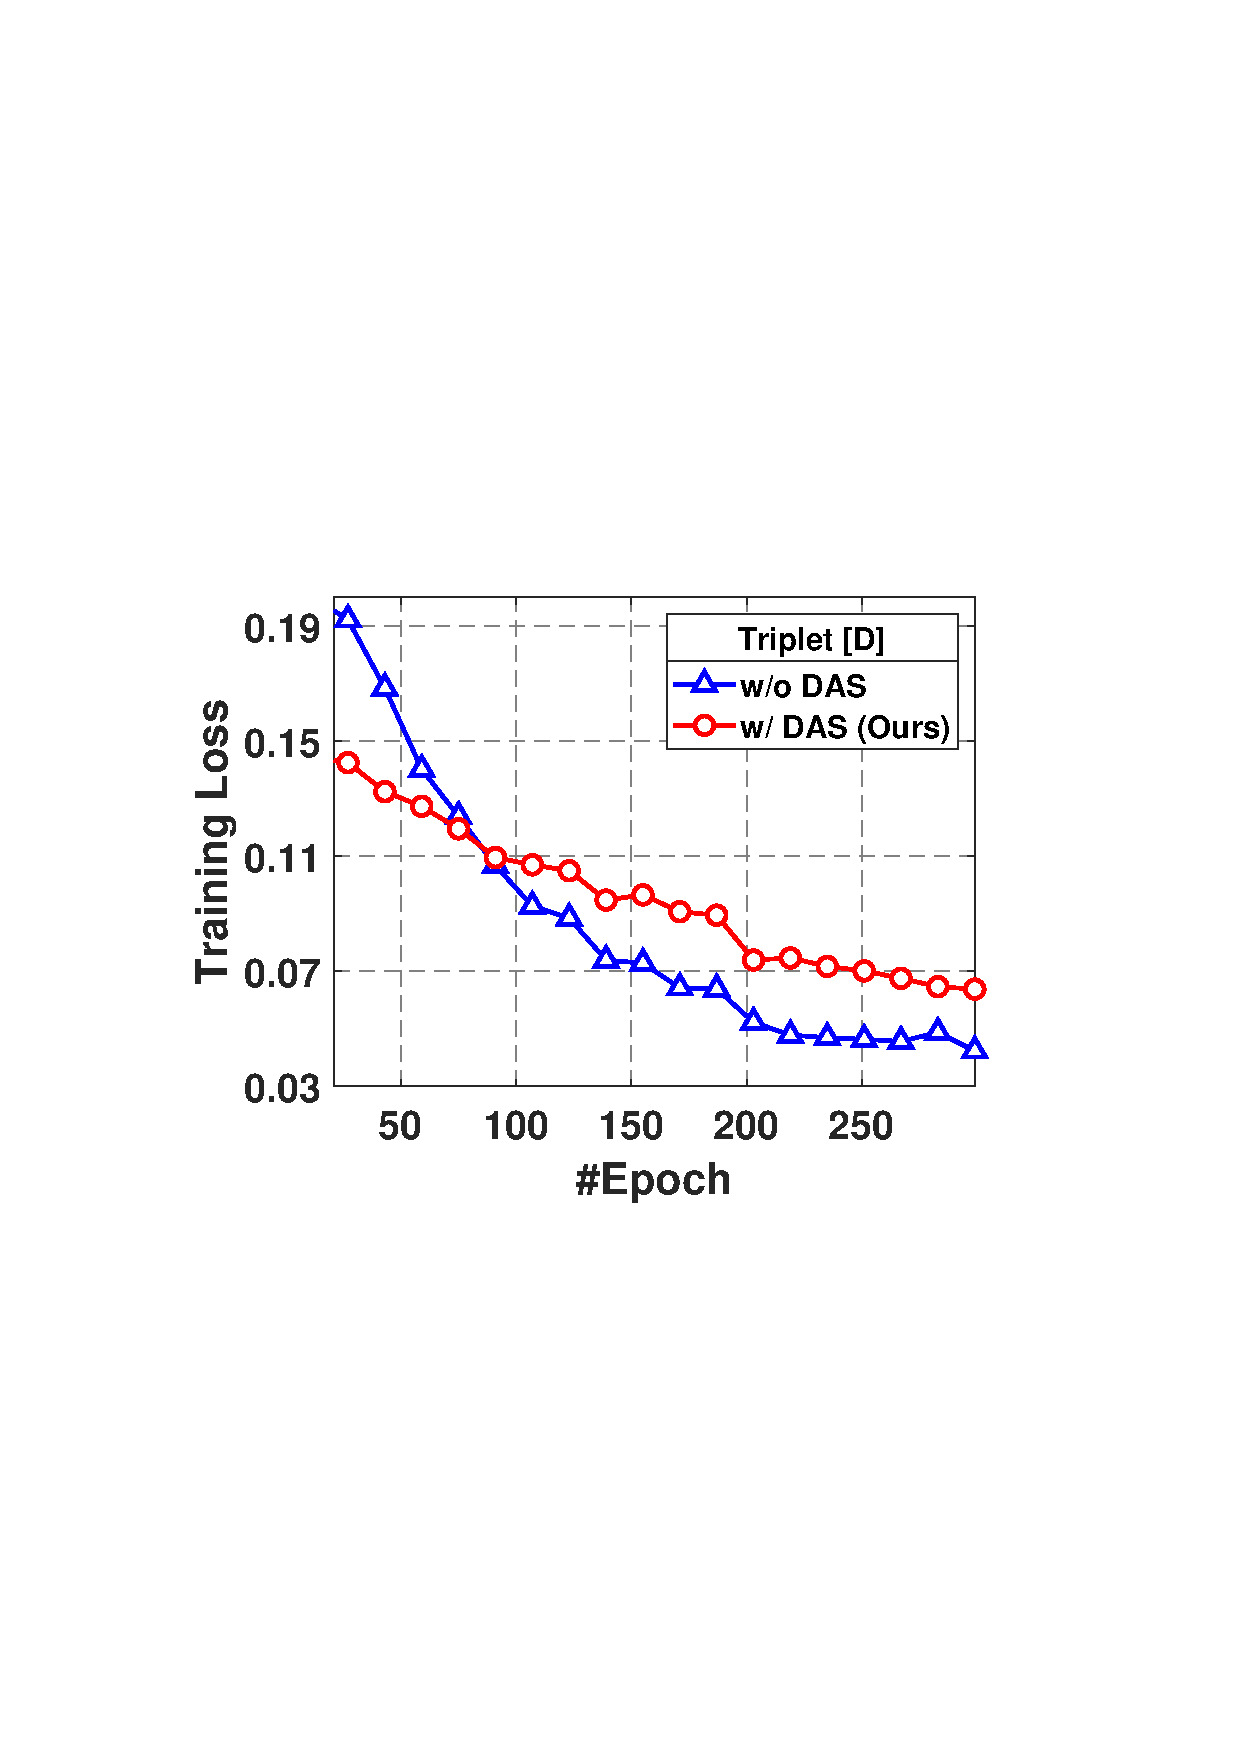
\includegraphics[width=.48\linewidth]{images/TripletD_loss.pdf}
        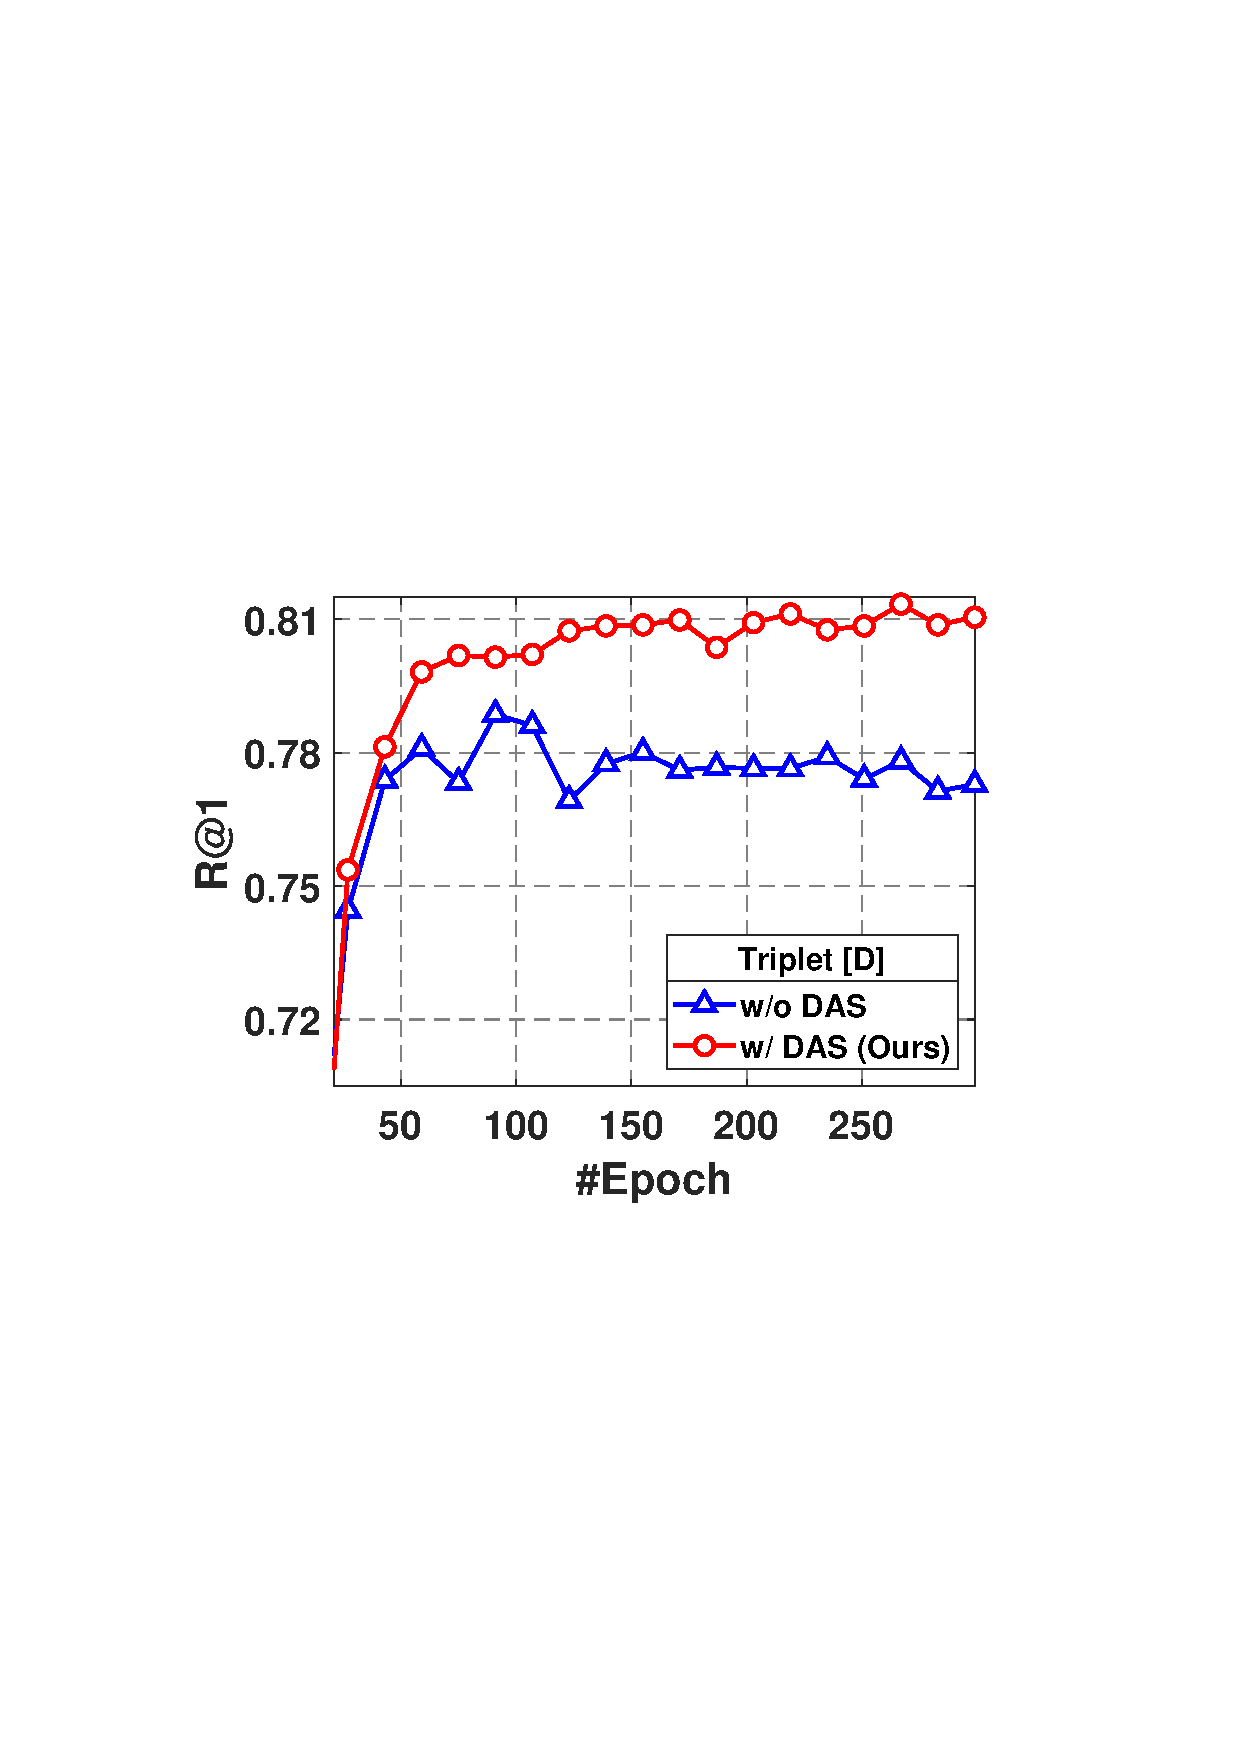
\includegraphics[width=.48\linewidth]{images/TripletD_recall1.pdf}
    \end{minipage}

    \vspace{0.5em}
    \centering
    \textbf{\color{blue}Image Retrieval Results:}

    \centering
    \vspace{0.2em}
    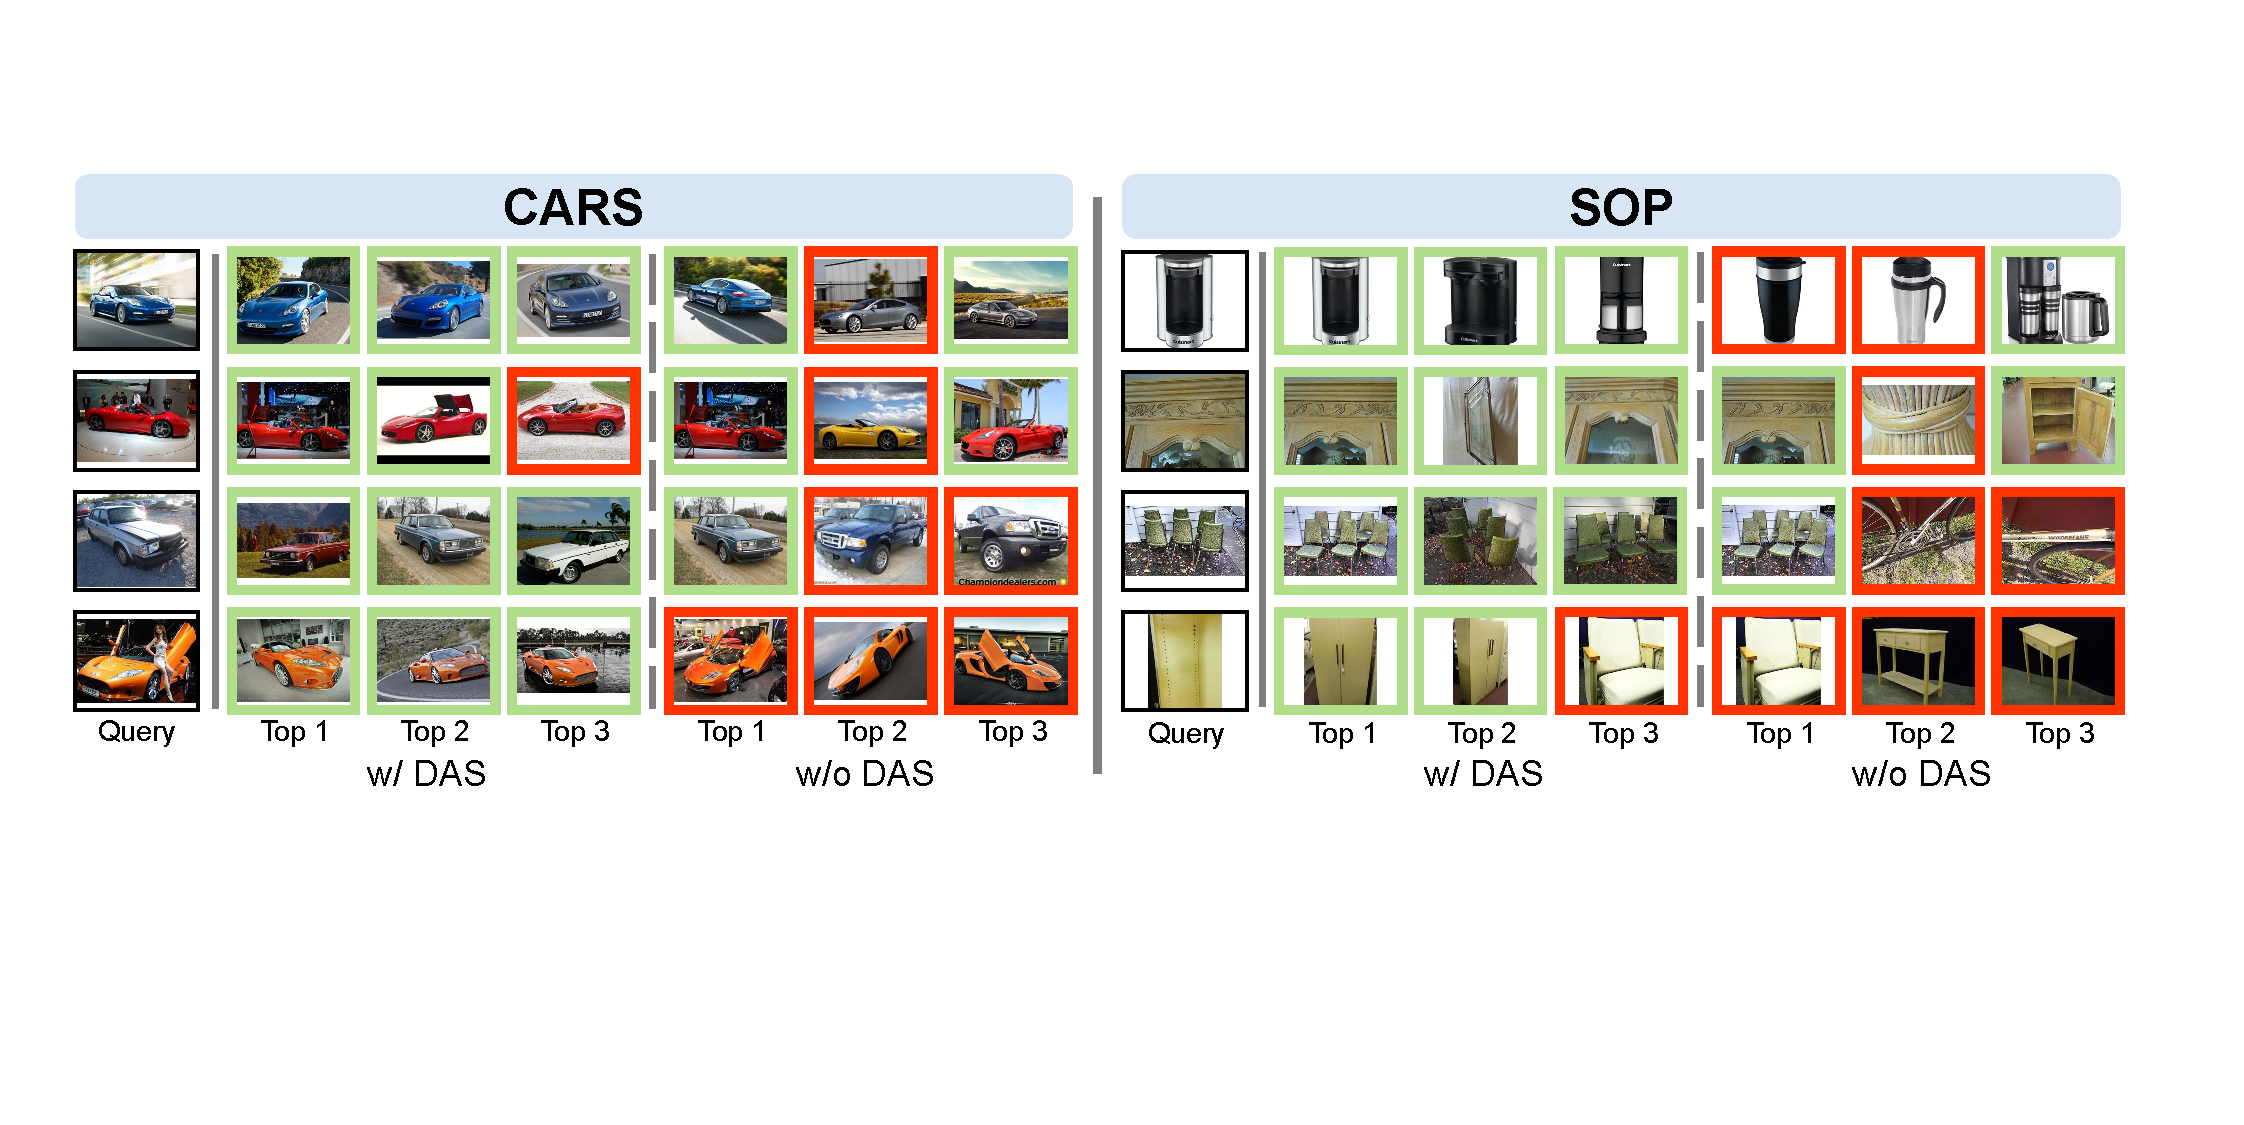
\includegraphics[width=.9\linewidth]{images/cars_sop_compare.pdf}
        
    \vspace{-1.0em}
    \begin{flushleft}
    \begin{minipage}[t]{0.5\linewidth}
        % \centering
        % \textbf{\color{blue}Ablation studies:}

        % \vspace{0.3em}
        % \newcommand{\improve}{\textbf}
\resizebox{.75\textwidth}{!}{ 
% \huge
\begin{tabular}{cclll}
    \toprule
    \shortbfs & \shorttmb & R@1 & F1 & NMI \\
    \midrule
    &  &  78.86 & 35.80 & 65.85 \\
    \checkmark &  &  81.28 \improve{(+2.42)} & 36.22 \improve{(+0.42)} & 66.84 \improve{(+0.99)} \\
    & \checkmark &  81.83 \improve{(+2.97)} & 38.26 \improve{(+2.46)} & 67.81 \improve{(+1.96)} \\
    \checkmark & \checkmark &  82.63 \improve{(+3.77)} & 39.14     \improve{(+3.34)} & 68.12 \improve{(+2.27)} \\
    \bottomrule
\end{tabular}
}
        \centering
        \textbf{\color{blue}Comparisons with Proxy-based Approaches:}

        \vspace{0.3em}
        \resizebox{0.9\linewidth}{!}{
    \begin{tabular}{l|ccc|ccc|ccc}
        \toprule
        \multirow{2}[0]{*}{Method} & \multicolumn{3}{c|}{CUB} & \multicolumn{3}{c|}{CARS} & \multicolumn{3}{c}{SOP} \\ \cline{2-10}
        & R@1 & F1 & NMI & R@1 & F1 & NMI & R@1 & F1 & NMI \\
        \midrule
        Softmax & 61.58 & 36.12 & 66.73 & 79.07 & 37.11 & 67.01 & 77.92 & 37.20 & 90.05 \\
        Softmax~{+ \shortname} & \textbf{62.02} & \textbf{36.24} & \textbf{67.42} & \textbf{81.23} & \textbf{39.95} & \textbf{68.91} & \textbf{79.36} & \textbf{38.72} & \textbf{90.40}  \\
        \midrule
        ArcFace & 61.56 & 35.73 & 66.83 & 79.50 & 37.75 & 67.82 & 78.08 & 37.79 & 90.18 \\
        ArcFace~{+ \shortname} & \textbf{62.80} & \textbf{37.63} & \textbf{67.80} & \textbf{82.22} & \textbf{40.82} & \textbf{69.82} & \textbf{78.12} & \textbf{38.08} & \textbf{90.26} \\
        \bottomrule
    \end{tabular}
}
    \end{minipage}
    \end{flushleft}
    
    \begin{flushright}
    \vspace{-8.0em}
        \begin{minipage}{0.53\linewidth}
        \begin{flushright}
            \small
            \textbf{More details:} \url{https://github.com/lizhaoliu-Lec/DAS} \\ 
            \textbf{Contact:} \url{{selizhaoliu, sevtars}@mail.scut.edu.cn}
        \end{flushright}
        \end{minipage}
        \begin{minipage}{0.06\linewidth}
            \begin{center}
                
\includegraphics[width=\linewidth]{images/DAS-code.png}
            \end{center}
        \end{minipage}
        
        \begin{minipage}{0.45\linewidth}
             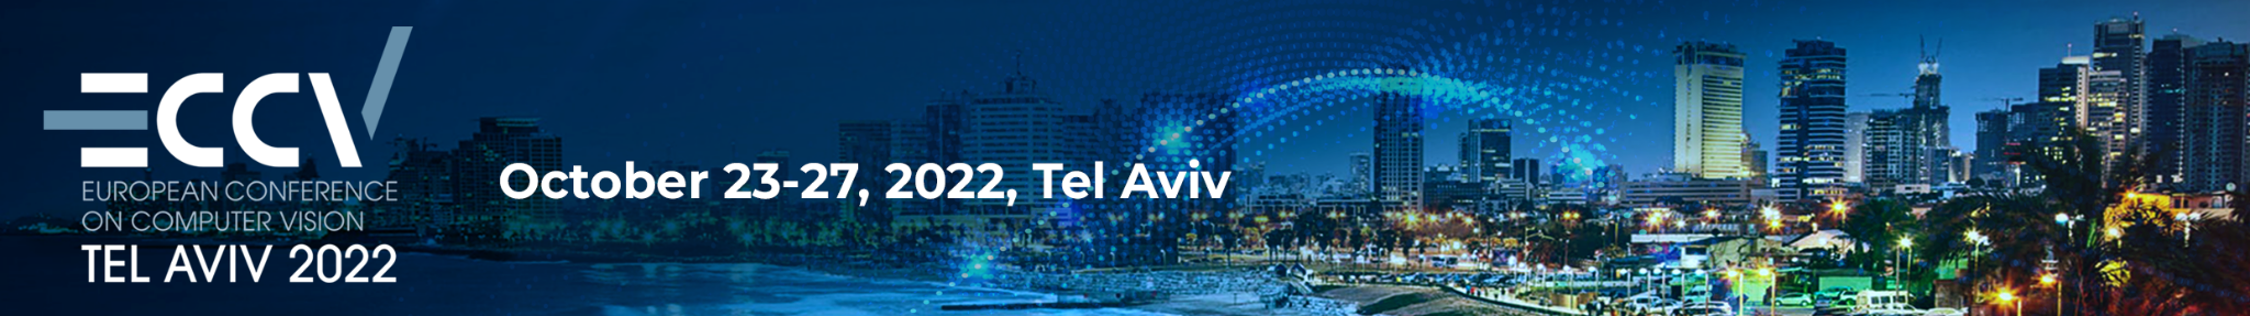
\includegraphics[width=\linewidth]{images/eccv-landscape.png}
        \end{minipage}
    \end{flushright}

}


%%%%%%%%%%%%%%%%%%%%%%%%%%%%%%%%%%%%%%%%%%%%%%%%%%%%%%%%%%%%%%%%%%%%%%%%%%%%%
\headerbox{\bf\color{blue} Problem Formulation}{name=formulation,column=0,row=0,below=contribution,span=2}{
    \begin{minipage}[t]{0.48\linewidth}
    
    \vspace{-8.5em}
    \textbf{\color{blue}Motivations:} 
     \begin{itemize}
        \item The basic hypothesis of metric learning: Embeddings close to each other in the embedding space have similar semantics.
        \item The missing embedding issue: The embedding space often has a barren area due to the absence of data points.
     \end{itemize}
      
    \end{minipage}
    \hfill
    \begin{minipage}[t]{0.48\linewidth}
    \begin{center}
        % \vspace{-0.8em}
        \centering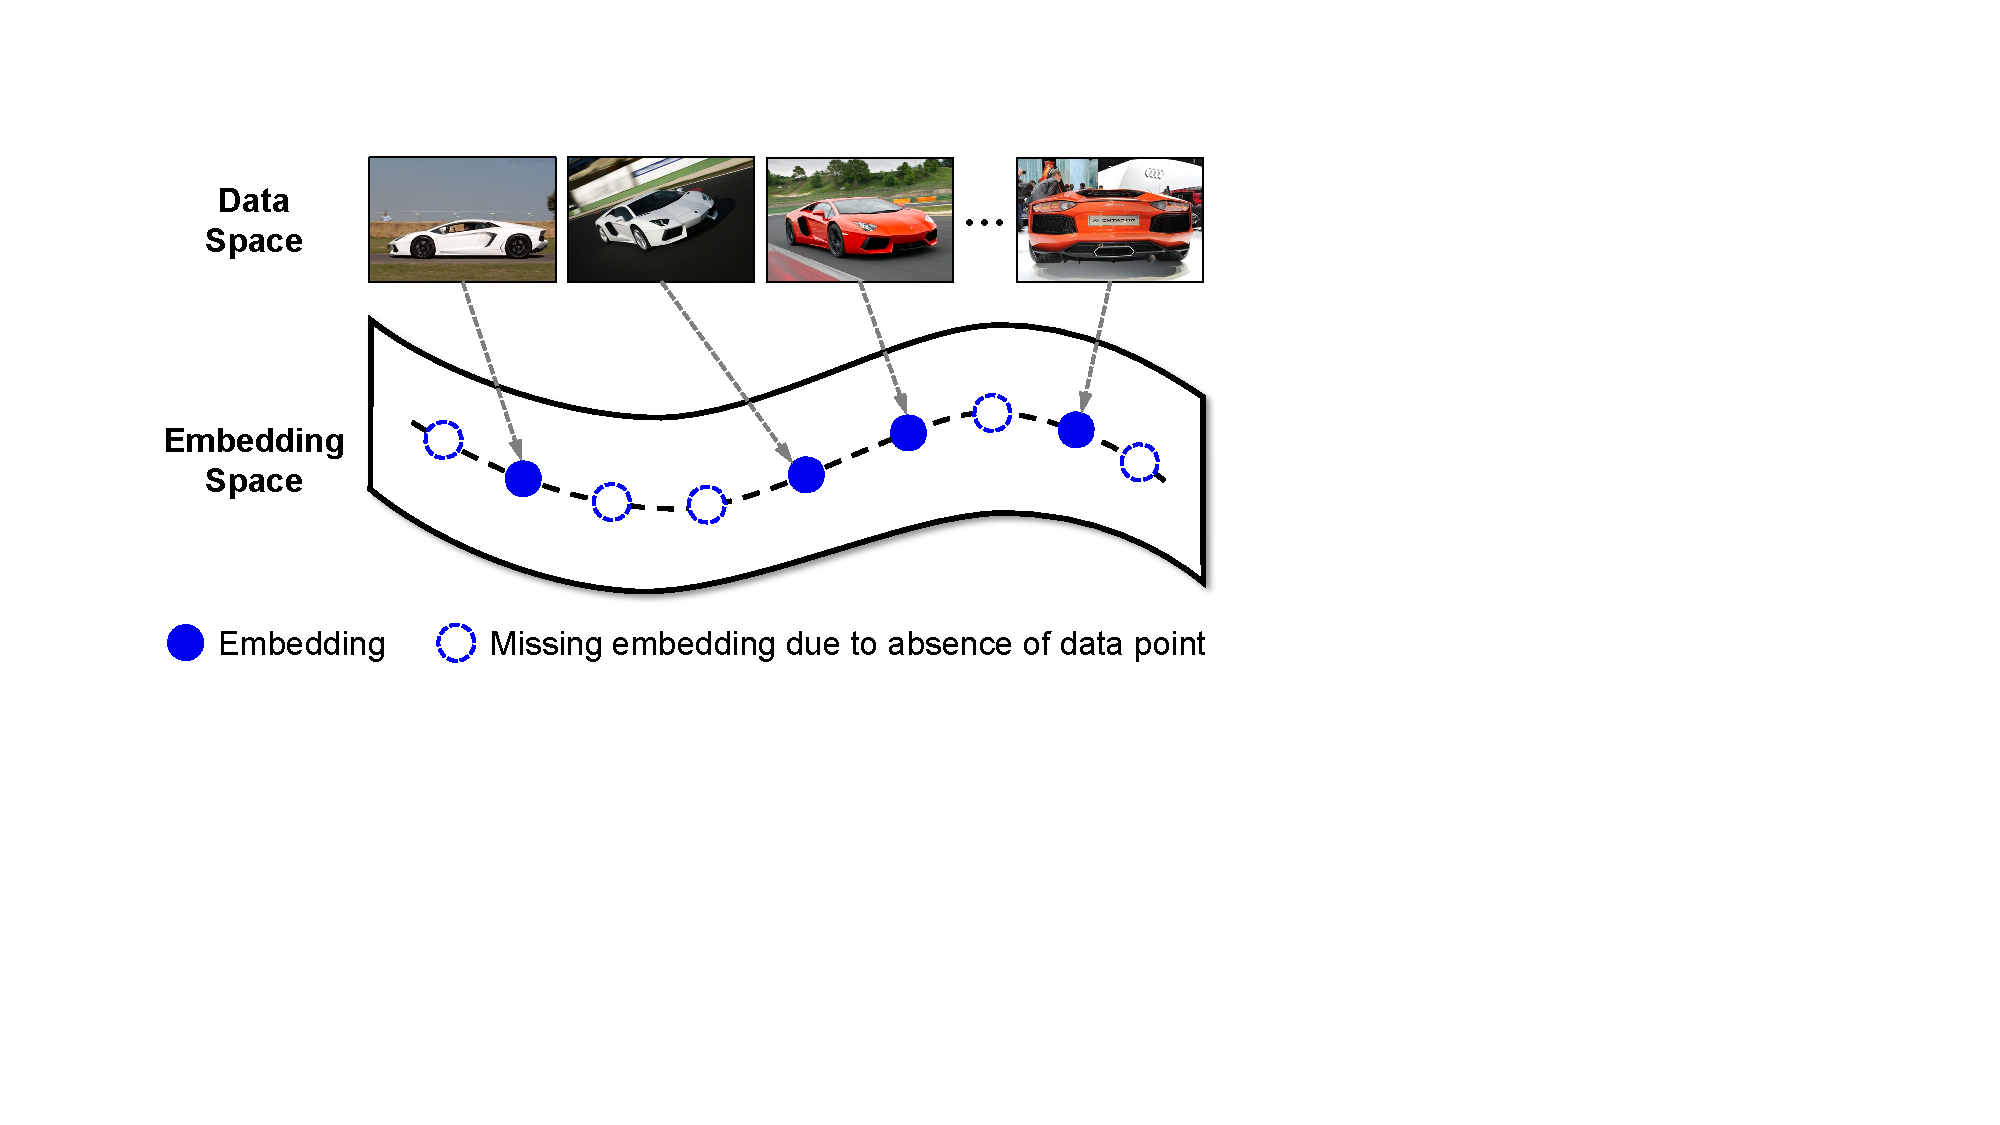
\includegraphics[width=\linewidth]{images/motivationV8.pdf}
    \end{center}
    % \vspace{0.2em}
    \end{minipage}
    
    \textbf{\color{blue}Main Idea:} Considering the embeddings $\bv$ with data points as anchor points, we alter anchor points semantics by semantic scaling and shifting to produce embedding $\bv'$:
    \vspace{-0.5em} 
    \begin{equation}
        \bv' = \operatorname{\shortname}(\bv;~\bs, \bb) = \underbrace{\bs~\odot~\bv}_\emph{scaling}\underbrace{+~~\bb}_\emph{shifting},
    \vspace{-0.2em} 
    \end{equation}
    where $\bs$ and $\bb$ denote the semantic scaling and shifting factors, respectively.
}

%%%%%%%%%%%%%%%%%%%%%%%%%%%%%%%%%%%%%%%%%%%%%%%%%%%%%%%%%%%%%%%%%%%%%%%%%%%%%
\headerbox{\bf\color{blue} Method}{name=abstract,column=0,below=formulation,span=2}{
  \shortname comprises two parts, namely a discriminative feature scaling for producing semantic scaling factors, and a memorized transformation for producing semantic shifting factors.
  \vspace{-0.2em}
  \begin{center}
   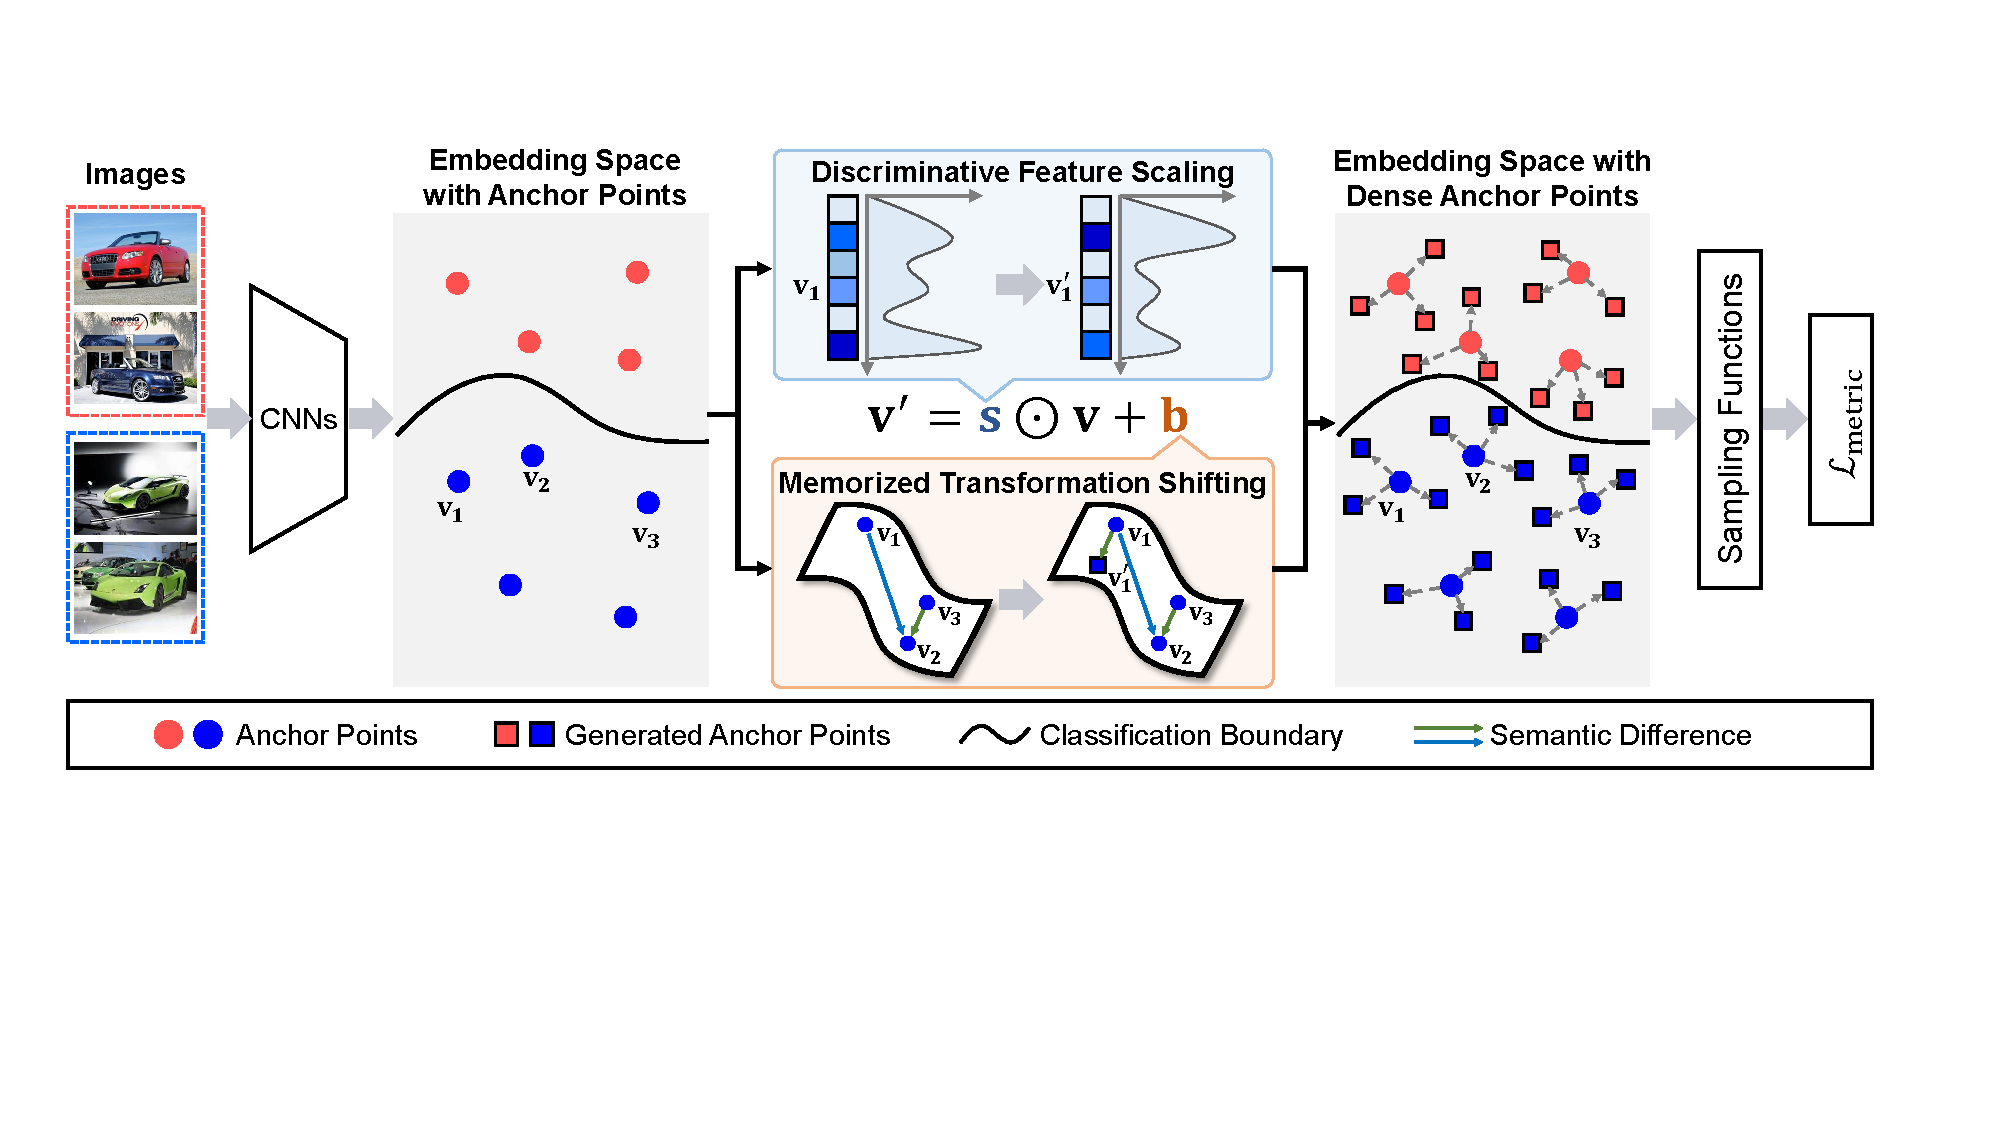
\includegraphics[width=0.85\textwidth]{images/frameworkV8.pdf}
  \end{center}
  \vspace{-0.5em}
  \begin{minipage}[t]{0.48\linewidth}
    \textbf{\color{blue}\bfs:}
    \vspace{-0.5em}
    \begin{equation}
        \bs = \bgamma \odot \bM[y_{\bv}] ~+~\mathbf{1}^d \odot (1 - \bM[y_{\bv}]),
    \end{equation} 
    \begin{itemize}
        \vspace{-0.5em}
        \item $\bs$ is the semantic scaling factor. 
        \item $\bM \in \mmR^{c \times d}$, a binary mask, records the frequently activated neurons for each class.
        \item $\bgamma \sim \operatorname{Uniform}[1 - r_s, 1 + r_s]^d$ and $r_s \in (0, 1)$ is a hyper-parameter.
    \end{itemize}
  \end{minipage}
  \hfill
  \begin{minipage}[t]{0.48\linewidth}
    \textbf{\color{blue}\tmb:}
    \vspace{-0.5em}
    \begin{equation}
        \label{eqn:shifting}
        \bb = r_b \bt, ~~ \bt \sim \{\bB[y_{\bv}, z]~\mid~z \small{=} {1, 2, \dots, Z}\}.
    \end{equation}
    \begin{itemize}
        \vspace{-0.5em}
        \item $\bb$ is the semantic shifting factor.
        \item $\bB$ is the memory bank that records the intra-class transformations according to the FIFO principle.
        \item $r_b \in (0, +\infty)$ is a hyper-parameter.
    \end{itemize}
  \end{minipage}

}


\end{poster}
\end{document}
